%%%%%%%%%%%%%%%%%%%%%%%%%%%%%%%%%%%%%%%%%%%%%%%%%%%%%%%%%%%%%%%%%%%%%%
%%
%%    PRELIMINARES
%%
%%%%%%%%%%%%%%%%%%%%%%%%%%%%%%%%%%%%%%%%%%%%%%%%%%%%%%%%%%%%%%%%%%%%%%

\chapter*{Preliminares}
\markboth{Preliminares}{Preliminares}
\addcontentsline{toc}{chapter}{Preliminares}


\par
\begin{floatingfigure}[l]{30mm}
\begin{center}
  \psfrag{s}{$s$}
  \psfrag{t}{$t$}
  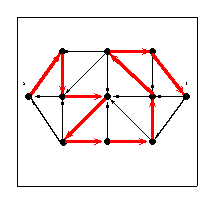
\includegraphics{./figs/rede}
\end{center} 
\end{floatingfigure}
\noindent


%\section{Grafos, passeios e caminhos}


Esto descritos nesta seo os ingredientes bsicos que envolvem os
problemas que sero tratados. A notao bsica que utilizamos  a de
Paulo Feofillof~\cite{pf:aula}

Um \defi{grafo}\index{grafo}  um objeto da forma $(V,A)$, 
onde $V$  um conjunto finito e $A$  um conjunto de pares ordenados 
de elementos de $V$. 

Os elementos de $V$ so chamados \defi{vrtices}\index{vrtices@vrtices} e os
elementos de $A$ so chamados \defi{arcos}\index{arcos}.  Para cada arco
$(u,v)$, os vrtices $u$ e $v$ representam a ponta inicial e a ponta final de
$(u,v)$, respectivamente.  Um arco $(u,v)$ tambm poder ser representado por
$uv$.

Um grafo  \defi{simtrico}\index{grafo!simtrico@simtrico} 
se para cada arco $uv$ existir tambm o arco $vu$. Diremos s vezes
que o arco $vu$  \defi{reverso}\index{arco!reverso}
 do arco $uv$ e que o par $\{(u,v),(v,u)\}$  uma \defi{aresta}\index{aresta}.
 
Um grafo pode ser naturalmente representado atravs de um
diagrama, como o da figura~\ref{fig:grafo}, onde os vrtices so
pequenas bolas e os arcos so as flechas ligando estas bolas. 

\begin{figure}[htbp]
 \begin{center}
    \psfrag{(a)}{$\iten{a}$}
    \psfrag{(b)}{$\iten{b}$}
    \psfrag{(c)}{$\iten{c}$}
    \psfrag{(d)}{$\iten{d}$}
    \psfrag{a}{{$a$}}
    \psfrag{b}{{$b$}}
    \psfrag{c}{{$c$}}
    \psfrag{d}{{$d$}}
    \psfrag{e}{{$e$}}   
    \psfrag{f}{{$f$}}
  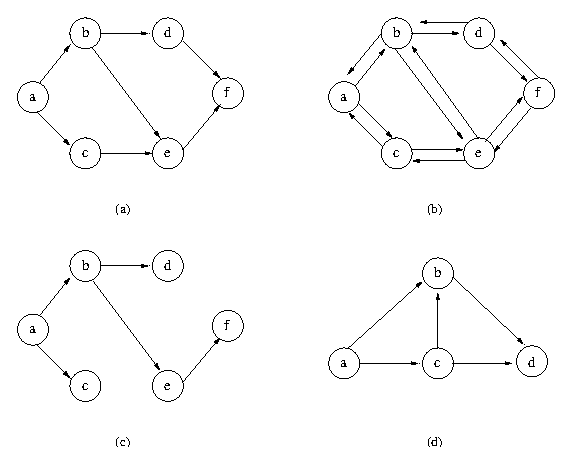
\includegraphics{./figs/grafo.eps}
  \caption{\label{fig:grafo} $\iten{a}$, $\iten{b}$, $\iten{c}$ e 
    $\iten{d}$ so exemplos de grafos. $\iten{b}$  um grafo simtrico.}
 \end{center}
 \end{figure}

%%% Passeio 
 Um \defi{passeio}\index{passeio} num grafo $(V,A)$  qualquer seqncia da forma
 \begin{eqnarray}
 \label{passeio}
 \seq{v_{0}, a_{1}, v_{1}, \ldots, a_{t}, v_{t}}
 \end{eqnarray}
onde $v_{0}, \ldots, v_{t}$ so vrtices, $a_{1}, \ldots, a_{t}$ 
so arcos e, para cada $i$, $a_{i}$  o arco $v_{i-1}v_{i}$. 
O vrtice
$v_{0}$  o \defi{incio} ou \defi{ponta inicial} do passeio
e o $v_{t}$  seu \defi{trmino} ou \defi{ponta final}.
%Uma \defi{passeio no-orientado}\index{passeio! no orientado@no orientado}
% uma seqncia como (\ref{passeio}) onde,
%para cada $i$, $\alpha_{i}$  o arco $v_{i-1}v_{i}$ ou o arco
% $v_{i}v_{i-1}$. 
Na figura~\ref{fig:grafo}$\iten{a}$ a seqncia
$\seq{a, ab, b, be, e, ef, f, fd, d, db, b, be, e, ef, f}$  um passeio com incio em $a$ e 
 trmino em $f$.
% e a seqncia $\seq{a, ac, c, ce, e, be, b, bd, d,df,f}$
%  um passeio no-orientado com incio em $a$ e trmino em $f$. 

%%%% 
Se $P:=\seq{v_{0}, a_{1}, v_{1}, \ldots, a_{t}, v_{t}}$, ento qualquer 
subseqncia da forma  
 \begin{eqnarray}
  \label{subpasseio}
   \seq{v_{i}, a_{i+1}, v_{i+1}, \ldots, a_{j}, v_{j}}
 \end{eqnarray}
com $0 \leq i \leq j \leq t$ ser um \defi{sub-passeio} de $P$. 
Alm disso, se $i=0$,  ento o sub-passeio ser dito um 
\defi{prefixo} de $P$.
Na figura~\ref{fig:grafo}$\iten{a}$ a seqncia $\seq{a, ab, b, be, e, ef, f,
fd, d}$  um sub-passeio e prefixo de do passeio 
$\seq{a, ab, b, be, e, ef, f, fd, d, db, b, be, e, ef, f}$.


%%% Caminhos
Um \defi{caminho}\index{caminho}  um passeio
sem vrtices repetidos.
%Um \defi{caminho no-orientado}\index{caminho!no-orientado@no-orientado} 
% um passeio no-orientado sem vrtices repetidos.
Na figura~\ref{fig:grafo}$\iten{a}$ a seqncia
 $\seq{a, ab, b, be, e, ef, f}$  um caminho com incio em $a$ e 
 trmino em $f$.
% e a seqncia $\seq{a, ac, c, ce, e, be, b, bd, d, df,
% f}$  um caminho no-orientado com incio em $a$ e trmino em $f$. 

 
%
% funo custo
%

Uma \defi{funo custo}\index{funo@funo!custo}\index{custo} em
$(V,A)$  uma funo de $A$ em $\NonnegInt$. Se $c$ for uma funo
custo em $(V,A)$ e $uv$ estiver em $A$, ento
$c(u,v)$ ser o valor de $c$ em $uv$. 
%
% Custo de um passeio e passeio de custo mnimo.
% 
Se $P$ for um passeio em um grafo $(V,A)$ e $c$ uma funo custo, 
denotaremos por $c(P)$ o \defi{custo do caminho} $P$%
\index{custo do caminho}, ou seja, $c(P)$  o somatrio dos custos
de todos os arcos em $P$.  Um passeio $P$ tem \defi{custo mnimo} se
$c(P) \leq c(P')$ para todo passeio $P'$ que tenha o mesmo incio e trmino
que $P$. Um passeio de custo mnimo  comumente chamado de \defi{caminho
mnimo}.
 
%
% Problema dos menores caminhos 
% 
 
Um problema fundamental em otimizao combinatria que tem um papel de
destaque neste projeto  o 
\defi{problema do caminho mnimo}, denotado por
\PCM:\index{problema!do caminho mnimo@do caminho mnimo}
 \begin{quote}
   \textbf{Problema} \PCM$(V,A,c,s,t)$: 
   \index{\PCM}\mar{\PCM}
%%%%%%%%%%%%%%%%%%%%%%%%%%%%%%%%%%%%%%%%%%%%%%%%%%%%%%%%%%%%%%%%%%%
   Dado um grafo $(V,A)$, uma funo
   custo~$c$ e dois vrtice $s$ e $t$, 
   encontrar um caminho de custo mnimo 
   de $s$ a~$t$.
 \end{quote}
Na literatura essa verso  conhecida como \textit{single-pair shortest path
problem}\index{single-pair shortest path@single-source shortest path}. 
O celebrado algoritmo de Edsger Wybe Dijkstra~\cite{dijkstra59:note} 
resolve o problema do caminho mnimo.



Denotaremos, quando no houver
ambigidade, por $n$ e $m$ os nmeros $|V|$ e $|A|$, respectivamente.
Alm disso, representaremos por $T(n,m)$ o consumo de tempo de uma
subrotina genrica para resolver o \PCM\ em um grafo com $n$ vrtices
e $m$ arestas.
O algoritmo mais eficiente  conhecido para o \PCM\ foi 
projetado por Michael L. Fredman e Robert Endre
Tarjan~\cite{FredTarjan:Fibonacci}
e consome tempo $\Oh(m + n \log n)$. Existe ainda um algoritmo que consome
tempo linear \textit{sob um outro modelo de computao} que foi
desenvolvido por Mikkel Thorup~\cite{thorup:sssp-1999}.    
